%\documentclass[20pt,-letter paper]{article}
%\usepackage{amsmath}
%\usepackage{gensymb}
%\usepackage{mathtools}
%\providecommand{\brak}[1]{\ensuremath{\left(#1\right)}}
%\title{}
%\author{Prof.G V V sharma}
%\date{\today}

%\begin{document}

%\maketitle{Questions}

\begin{enumerate}
\item Find the sum and product of zeroes of the polynomial $p(x)=x^2+5x+6$
\item If $2\cos  \theta = \sqrt{3}$ , then find the value of $\theta$
\item Find the discriminant of the quadratic equation $2x^2-5x-6=0$.
\item  In $\triangle ABC$, right-angled at $A$, if $AB=7 cm$ and $AC=24 cm$, then find $\sin B$
and $\tan C$.

\item \begin{enumerate}

\item If  $\sin (A+B) = \sqrt{3}/2,
 \sin (A-B) = 1/2,$ Where $0\degree<A+B<90\degree; A>B$, then find the values of $A$ and $B$.

\item  Simplify :
\begin{align}
\frac{\sin 30\degree + \tan 45\degree-\cos 60\degree}{\sec 30\degree + \cos 60\degree + \cot 45\degree} 
\end{align}
\end{enumerate}


\item The greater of two supplementary angles exceeds the smaller by $18\degree$. Find the two angles.

\item  Prove that $7 \sqrt{2}$ is an irrational number ,given that $\sqrt{2}$ is an irrational number.

\item \begin{enumerate}
\item Prove that :
\begin{align}
 \sec \theta (1-\sin\theta)(\sec\theta+ \tan\theta)=1
\end{align}

\item Prove that :
\begin{align}
\frac{1+\sec A}{\sec A}=\frac{\sin^2 A}{1-\cos A} 
\end{align}
\end{enumerate}

\item If $\alpha,\beta$ are the zeroes of the quadratic polynomial $x^2+9x+20$, from a quadratic polynomial whose zeroes are  $(\alpha+1)$ and 
$(\beta+1)$.


\item \begin{enumerate}
\item The diagonal of a rectangular field is $60$ meters more than the shorter side, find the sides of the field.


\item The sum of the ages of a father and his son is $45$ years. Five years ago, the product of their ages (in years) was $124 $. Determine their present ages

\end{enumerate} 


\item Write a quadratic polynomial sum of Whose zeroes is $-5
$ and product is $6$.



\item If the sum of the zeroes of the polynomial $2x^2-3ax+4$ is $6$, then the value of a 
\begin{enumerate}
\item $4$
\item $-4$
\item $2$
\item $-2$
\end{enumerate}

\item The common zero of the polynomials $x^3+1, x^2-1$ and $x^2+2x+1$ is 
\begin{enumerate}
\item $-2$
\item $-1$
\item  $1$
\item  $2$
\end{enumerate}

\item If $\alpha,\beta$ are the zeroes of the polynomial $x^2 - 4x+6$, then the value of $\alpha\beta$ is
\begin{enumerate}
\item $4$
\item $-4$
\item $6$
\item $-6$
\end{enumerate}

\item The zeroes of the polynomial $3x^2-5x-2$ are 
\begin{enumerate}
\item $\frac{1}{3}$,$2$
\item $-\frac{1}{3}$,$2$
\item $\frac{1}{3}$,-$2$
\item $-\frac{1}{3}$,-$2$
\end{enumerate}

\item If is a zero of the polynomial $p(x)=ax^2-3(a-1)x-1$  then the value of a is 
\begin{enumerate}
\item $\frac{1}{3}$,$2$
\item $-\frac{1}{3}$,$2$
\item $\frac{1}{3}$,-$2$
\item $-\frac{1}{3}$,-$2$
\end{enumerate}



\item If  $\tan \theta = 4/3$, find the value 
$\frac{2\sin \theta -3\cos \theta}{2\sin\theta+3\cos\theta}$

\item If x=  $a\cos\theta$ and y=$b\sin\theta$, then find the value of   $b^2x^2+a^2y^2$

\item A number consists of two digits whose sum is $9$. if $27$ is added to the number, the digits are reversed. Find the number
\item Prove that :
\begin{align}
\frac{\tan\theta-\cot\theta}{\sin\theta\cos\theta}=\tan^2\theta-\cot^2\theta 
\end{align}
\item Prove that:
\begin{align}
(\sec\theta-\tan\theta)^2 =\frac{1+\sin\theta}{1-\sin\theta}
\end{align}

\item The sum of the squares of three consecutive positive 
integers is $110$. Find the positive integers.

\item Ram can row a boat at the rate of $4$ km/hour in still 
water. If he takes $8$ hours in going $12$ km upstream and 
$12$ km downstream, find the speed of the stream.
	\item Write the quadratic equation in $x$ whose roots are $2$ and $-5$.
		\item If $\alpha$ and $\beta$ are zeros of the quadratic polynomial $f(x) = x^2 - x - 4$, find the value of $\frac{1}{\alpha} + \frac{1}{\beta} - {\alpha \beta}$.
		\item If one zero of the quadratic polynomial $x^{2} + 3x + k$ is $2$, then find the value of $k$.
		\item If $3\sin A = 1$, then find the value of $\sec A$.
		\item Show that: $\frac{1 + \cot^2{\theta}}{1 + \tan^2{\theta}} = \cot^2{\theta}$.
\item Simplify :$${\csc^{2}{60\degree} \sin^{2}{30\degree} - \sec^{2}{60\degree}}$$
	\item If $\tan{\theta} + \cot{\theta}$ = $\frac{4 \sqrt{3}}{3}$, then find the value of $\tan^{2}{\theta} + \cot^{2}{\theta}$. 
	\item Divide the polynomial $f(x) = 5x^{3} + 10x^{2} - 30{x} - 15$ by the polynomial $g(x) = x^{2} + 1 + x$ and hence, find the quotient and the remainder.
		\item Prove:$$\frac{1}{(\cot A)(\sec A) - \cot A} - \csc A = \csc A - \frac{1}{(\cot A)(\sec A) + \cot A}$$
		\item Prove:$$\sin^{6} A + 3\sin^{2} A \cos^{2} A = 1 - \cos^{6}  A$$
		\item One of the root of the quadratic equation $2x^{2} - 8x - k = 0$ is $\frac{5}{2}$. Find the value of $k$, Also find the root.
		\item Using quadratic formula, solve the following equation for x:$$abx^{2} + (b^{2} - ac)x - bc = 0$$.
	\item With vertices A,B and C of a triangle ABC as centers, arcs are drawn with radii $2$ cm each as/ shown in the figure. If AB = $6$ cm, BC = $8$ cm and AC = $10$ cm, find the area of the shaded region.	  	
	\begin{figure}[h]
	      			\centering
	      			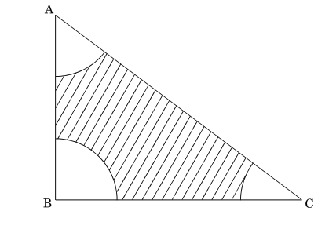
\includegraphics[width=\columnwidth]{figs/triashaded.jpg}
				\caption{}
				\label{fig:xxxx}
      \end{figure}
	\item Water is being pumped out through a circular pipe whose internal diameter is $8$ cm. If the rate of flow of water is $80$ cm/s, then how many liters of water is being pumped out through this pipe in one hour ?
		\item A man on the top of a vertical tower observes a car moving at a uniform speed coming directly towards it. If it takes $18$ minutes for the angle of depression to change from $30\degree$ to $60\degree$, how soon after this will the car reach the tower ?

		\item A girl on a ship standing on a wooden platform, which is $50$ m above water level, observes the angle of elevation of a top of a hill as $30\degree$ and the angle of depression of the base of the hill as $60\degree$. Calculate the distance of the hill from the platform and the height of the hill.
\end{enumerate}

%\end{document}
